%%
%% This is file `sample-sigconf.tex',
%% generated with the docstrip utility.
%%
%% The original source files were:
%%
%% samples.dtx  (with options: `sigconf')
%% 
%% IMPORTANT NOTICE:
%% 
%% For the copyright see the source file.
%% 
%% Any modified versions of this file must be renamed
%% with new filenames distinct from sample-sigconf.tex.
%% 
%% For distribution of the original source see the terms
%% for copying and modification in the file samples.dtx.
%% 
%% This generated file may be distributed as long as the
%% original source files, as listed above, are part of the
%% same distribution. (The sources need not necessarily be
%% in the same archive or directory.)
%%

\usepackage{enumitem}

%% The first command in your LaTeX source must be the \documentclass command.
\documentclass[sigconf]{acmart}
\settopmatter{printacmref=false}
%%
%% \BibTeX command to typeset BibTeX logo in the docs
\AtBeginDocument{%
  \providecommand\BibTeX{{%
    \normalfont B\kern-0.5em{\scshape i\kern-0.25em b}\kern-0.8em\TeX}}}

%% Rights management information.  This information is sent to you
%% when you complete the rights form.  These commands have SAMPLE
%% values in them; it is your responsibility as an author to replace
%% the commands and values with those provided to you when you
%% complete the rights form.
\setcopyright{iw3c2w3}
\copyrightyear{\the\year{}}
\acmYear{\the\year{}}


%%
%% end of the preamble, start of the body of the document source.
\begin{document}

%%
%% The "title" command has an optional parameter,
%% allowing the author to define a "short title" to be used in page headers.
\title{Exploring User Prompting Behavior in LLM Interactions}

%%
%% The "author" command and its associated commands are used to define
%% the authors and their affiliations.
%% Of note is the shared affiliation of the first two authors, and the
%% "authornote" and "authornotemark" commands
%% used to denote shared contribution to the research.
\author{Maximilian Slapnik}
%\orcid{1234-5678-9012}
\email{Maximilian.Slapnik@campus.lmu.de}
\affiliation{%
  \institution{LMU Munich}
  \city{Munich}
  \country{Germany}
}


%%
%% By default, the full list of authors will be used in the page
%% headers. Often, this list is too long, and will overlap
%% other information printed in the page headers. This command allows
%% the author to define a more concise list
%% of authors' names for this purpose.
%\renewcommand{\shortauthors}{Trovato and Tobin, et al.}

%%
%% The abstract is a short summary of the work to be presented in the
%% article.
\begin{abstract}
  Artificial Intelligence (AI) plays an increasingly important role in the daily lives of millions of people.
  Large Language Models (LLMs) are the most prominent implementation of AI that is used not only by experts, but equally by ordinary users as well.
  LLMs can respond to any textual input (prompts) with human-like answers, leveraging the training data that was used to implement the model.
  Even though prompting LLMs seems very straightforward, the question arises if it is possible to streamline the interactions with said models in order to optimize outputs.
  We explore the behavior of a randomized trial of 100 interactions of users with LLMs that are publicly available on ShareGPT.
  The goal of this investigation is the discovery of recurring patterns in behavior and the evaluation of human tendencies as well as biases of users when interacting with AI models in order to understand current behaviors and propose optimization opportunities.
\end{abstract}

%%
%% The code below is generated by the tool at http://dl.acm.org/ccs.cfm.
%% Please copy and paste the code instead of the example below.
%%
%\begin{CCSXML}
%<ccs2012>
%<concept>
%<concept_id>10003120.10003121.10003125.10011666</concept_id>
%<concept_desc>Human-centered computing~Touch screens</concept_desc>
%<concept_significance>500</concept_significance>
%</concept>
%</ccs2012>
%\end{CCSXML}
%
%\ccsdesc[500]{Human-centered computing~Touch screens}

%%
%% Keywords. The author(s) should pick words that accurately describe
%% the work being presented. Separate the keywords with commas.
%\keywords{datasets, neural networks, gaze detection, text tagging}

%% A "teaser" image appears between the author and affiliation
%% information and the body of the document, and typically spans the
%% page.
%\begin{teaserfigure}
%  \includegraphics[width=\textwidth]{figures/sampleteaser}
%  \caption{Seattle Mariners at Spring Training, 2010.}
%  \Description{Enjoying the baseball game from the third-base
%  seats. Ichiro Suzuki preparing to bat.}
%  \label{fig:teaser}
%\end{teaserfigure}

%%
%% This command processes the author and affiliation and title
%% information and builds the first part of the formatted document.
\maketitle


% 1. Introduction
\section{Introduction}

% 2. Background and Related Work
\section{Background and Related Work}
  \subsection{Large Language Models (LLMs)}
$\circ$ General information on LLMs, such as their workings, training data, text generation, real world usage, and current limitations
  \subsection{User Interaction with LLMs}
$\circ$ Description of LLM use cases and related work, primarily paying attention to ordinary frequent users as we lay a particular focus on daily, and not only expert usage

% 3. Study on Usage Patterns of LLM Users
\section{Study on Usage Patterns of LLM Users}
  \subsection{Intro and Research Objective}
$\circ$ Overview of the study goal, the methodology, and the individual steps that will be taken during its course
  \subsection{Research Method: ShareGPT}
$\circ$ Information on the ShareGPT platform, its user base, its suitability for the study, and which data we are going to use
  \subsection{Study Results}
    \subsubsection{Findings}
$\circ$ Listing of the results of the study, potentially segregated into categories that can be defined in advance
    \subsubsection{Observable Trends}
$\circ$ Objective analysis of results with a particular focus on observable trends in user behavior and data patterns

% 4. Discussion
\section{Discussion}
  \subsection{Observed Behaviour (Synthesis)}
$\circ$ Subjective evaluation of findings
    \subsubsection{Why do users interact with LLMs the way they do?}
$\circ$ Reasoning and informed assumptions on the causes of observed behavior
    \subsubsection{Prompt Improvement Possibilities}

$\circ$ Proposition of ways to enhance prompts as well as associated results, incorporating findings from related research
  \subsection{Outlook and Future Developments}
    \subsubsection{Auto-GPT}
$\circ$ Introduction to future developments in the realm of LLM interaction, such as AI-based agents which may execute prompts autonomously in the future
    \subsubsection{Prompt Engineering}
$\circ$ Focus on the newly emerging discipline of prompt engineering which is a direct result of the increased significance of LLMs and required competencies for successful interaction

% 5. Conclusion
\section{Conclusion}

%%%%%%%%%%%%%%%%%%%%%%%%%%%%%%% Introduction %%%%%%%%%%%%%%%%%%%%%%%%%%%%%%%

%%%%%%%%%%%%%%%%%%%%%%%%%%%%%%%%% Introduction %%%%%%%%%%%%%%%%%%%%%%%%%%%%%%%%%
\section{Introduction}
\label{sec:introduction}
%% refer to https://intra.ece.ucr.edu/~rlake/Whitesides_writing_res_paper.pdf for tips on introduction?
%% INTRO - TOPIC

%Why is the work important?
\sloppy % use sloppy to improve linebreaks - longer words do not overflow
Artificial Intelligence (AI) -based tools continually gain prominence as regularly leveraged tools in the
daily lives of millions of people.
Today, the significance of this technology is reflected in the current AI market size that is
estimated to be \$142 billion USD, and forecasted to increase more than tenfold by 2030~\cite{statista_artificial_2023}.
% TODO include some stats, such as daily ChatGPT users?
In addition to typical AI applications such as recommendation systems or autonomous agents, generative
models are notably increasing in popularity as well, making it one of the central research topics
in the field.
One of the most widely used implementations of generative models are Large Language Models (LLMs),
the most popular example at the moment being OpenAI's ChatGPT~\cite{openai_chatgpt_2023}.
Adoption rates of generative AI applications among professionals are increasing rapidly, and are
already at
around 30\%~\cite{statista_us_2022}.

Large Language Models are mainly implemented in the form of text generating chatbots that can
answer seemingly any question a user might pose.
Although no expert knowledge is required to formulate a prompt and interact with an LLM-based bot, it is challenging to optimize the output, since it varies depending on the structure, wording,
and composition of the input. %TODO cite?
Any form of model input, whether it is in the form of a task or a question, is commonly
referred to as \("\)prompting\("\) the model.
Due to the vast application possibilities and promising future developments of LLMs, exploration of
user prompting behavior in interactions with such models is of particular interest.
Plenty of research has been conducted in the field of user interactions with LLMs already,
mainly in regard to query reformulation strategies, studies of common user errors when prompting,
different prompt composition strategies, and general LLM limitations.

%- The objectives of the work.
In this paper, we are going to explain the fundamentals and workings of LLMs and prompting,
describe related research in the realm of user - LLM exchange, and perform our own investigation of
user behavior in such interactions.
This investigation has the objective of facilitating comprehension of existing challenges users
face when dealing with Large Language Models.
Furthermore, readers will gain a better understanding of the design of effective prompts that
enhance model output.

%- Guidance to the reader:
% What should the reader watch for in the paper?
% What are the interesting high points? What strategy did we use?
Since the main part of this paper will be complemented by an analysis of real-world examples, the
reader can expect to develop an enhanced comprehension of actual user prompting behavior.
To obtain these insights, we will leverage input data mainly gathered from the website
ShareGPT~\cite{sharegpt_sharegpt_2023},
which enables users to store conversations they have had with the ChatGPT model for later retrieval
or sharing them publicly.

% TODO add links (\ref) to sections
The paper is organized as follows.
This introduction is succeeded by a related work section that sets the context for all subsequent
parts by first focusing on Large Language Models (LLMs) and covering general information about
their workings, training data, text generation capabilities, real-world usage, and current limitations.
We then explore user interactions with LLMs, explain the concept of prompting, and highlight
various use cases as well as related research.

The next section introduces the study by outlining the research objective and
describing the methodology and individual steps that will be taken.
It then focuses on the research method we use, as well as the ShareGPT and Midjourney platforms,
which provide the input data for the study.

Subsequently, we present our findings.
To do so, we first list the study results, organized into predefined categories.
% TODO check if true
We then analyze observable trends in user behavior and data patterns.

The following discussion section starts with a synthesis of our observations.
We then go into more detail about the reasons why users interact with LLMs the way they do,
offering reasoning and informed assumptions.
Additionally, we explore possibilities for prompt improvements based on findings from related
research.

In the outlook section, we provide a perspective on future developments, divided into an
introduction of the concept of Auto-GPT as a possible future iteration of prompting, as well as an
overview of prompt engineering as a newly emerging discipline in the technology sector.

The final section of this paper offers a consolidation of the findings and associated discussions,
as well as a summary of how we could recognize findings from related research in our own input
samples.


%\section{Title Information}
%
%The title of your work should use capital letters appropriately -
%\url{https://capitalizemytitle.com/} has useful rules for
%capitalization. Use the {\verb|title|} command to define the title of
%your work. If your work has a subtitle, define it with the
%{\verb|subtitle|} command.  Do not insert line breaks in your title.
%
%If your title is lengthy, you must define a short version to be used
%in the page headers, to prevent overlapping text. The \verb|title|
%command has a ``short title'' parameter:
%\begin{verbatim}
%  \title[short title]{full title}
%\end{verbatim}
%
%\section{Authors and Affiliations}
%
%Each author must be defined separately for accurate metadata
%identification. Multiple authors may share one affiliation. Authors'
%names should not be abbreviated; use full first names wherever
%possible. Include authors' e-mail addresses whenever possible.
%
%Grouping authors' names or e-mail addresses, or providing an ``e-mail
%alias,'' as shown below, is not acceptable:
%\begin{verbatim}
%  \author{Brooke Aster, David Mehldau}
%  \email{dave,judy,steve@university.edu}
%  \email{firstname.lastname@phillips.org}
%\end{verbatim}
%
%The \verb|authornote| and \verb|authornotemark| commands allow a note
%to apply to multiple authors --- for example, if the first two authors
%of an article contributed equally to the work.
%
%If your author list is lengthy, you must define a shortened version of
%the list of authors to be used in the page headers, to prevent
%overlapping text. The following command should be placed just after
%the last \verb|\author{}| definition:
%\begin{verbatim}
%  \renewcommand{\shortauthors}{McCartney, et al.}
%\end{verbatim}
%Omitting this command will force the use of a concatenated list of all
%of the authors' names, which may result in overlapping text in the
%page headers.
%
%The article template's documentation, available at
%\url{https://www.acm.org/publications/proceedings-template}, has a
%complete explanation of these commands and tips for their effective
%use.
%
%Note that authors' addresses are mandatory for journal articles.
%
%\section{CCS Concepts and User-Defined Keywords}
%
%Two elements of the ``acmart'' document class provide powerful
%taxonomic tools for you to help readers find your work in an online
%search.
%
%The ACM Computing Classification System ---
%\url{https://www.acm.org/publications/class-2012} --- is a set of
%classifiers and concepts that describe the computing
%discipline. Authors can select entries from this classification
%system, via \url{https://dl.acm.org/ccs/ccs.cfm}, and generate the
%commands to be included in the \LaTeX\ source.
%
%User-defined keywords are a comma-separated list of words and phrases
%of the authors' choosing, providing a more flexible way of describing
%the research being presented.
%
%CCS concepts and user-defined keywords are required for for all
%articles over two pages in length, and are optional for one- and
%two-page articles (or abstracts).
%
%\section{Sectioning Commands}
%
%Your work should use standard \LaTeX\ sectioning commands:
%\verb|section|, \verb|subsection|, \verb|subsubsection|, and
%\verb|paragraph|. They should be numbered; do not remove the numbering
%from the commands.
%
%Simulating a sectioning command by setting the first word or words of
%a paragraph in boldface or italicized text is {\bfseries not allowed.}
%
%\section{Tables}
%
%The ``\verb|acmart|'' document class includes the ``\verb|booktabs|''
%package --- \url{https://ctan.org/pkg/booktabs} --- for preparing
%high-quality tables.
%
%Table captions are placed {\itshape above} the table.
%
%Because tables cannot be split across pages, the best placement for
%them is typically the top of the page nearest their initial cite.  To
%ensure this proper ``floating'' placement of tables, use the
%environment \textbf{table} to enclose the table's contents and the
%table caption.  The contents of the table itself must go in the
%\textbf{tabular} environment, to be aligned properly in rows and
%columns, with the desired horizontal and vertical rules.  Again,
%detailed instructions on \textbf{tabular} material are found in the
%\textit{\LaTeX\ User's Guide}.
%
%Immediately following this sentence is the point at which
%Table~\ref{tab:freq} is included in the input file; compare the
%placement of the table here with the table in the printed output of
%this document.
%
%\begin{table}
%  \caption{Frequency of Special Characters}
%  \label{tab:freq}
%  \begin{tabular}{ccl}
%    \toprule
%    Non-English or Math&Frequency&Comments\\
%    \midrule
%    \O & 1 in 1,000& For Swedish names\\
%    $\pi$ & 1 in 5& Common in math\\
%    \$ & 4 in 5 & Used in business\\
%    $\Psi^2_1$ & 1 in 40,000& Unexplained usage\\
%  \bottomrule
%\end{tabular}
%\end{table}
%
%To set a wider table, which takes up the whole width of the page's
%live area, use the environment \textbf{table*} to enclose the table's
%contents and the table caption.  As with a single-column table, this
%wide table will ``float'' to a location deemed more
%desirable. Immediately following this sentence is the point at which
%Table~\ref{tab:commands} is included in the input file; again, it is
%instructive to compare the placement of the table here with the table
%in the printed output of this document.
%
%\begin{table*}
%  \caption{Some Typical Commands}
%  \label{tab:commands}
%  \begin{tabular}{ccl}
%    \toprule
%    Command &A Number & Comments\\
%    \midrule
%    \texttt{{\char'134}author} & 100& Author \\
%    \texttt{{\char'134}table}& 300 & For tables\\
%    \texttt{{\char'134}table*}& 400& For wider tables\\
%    \bottomrule
%  \end{tabular}
%\end{table*}
%
%Always use midrule to separate table header rows from data rows, and
%use it only for this purpose. This enables assistive technologies to
%recognise table headers and support their users in navigating tables
%more easily.
%
%\section{Math Equations}
%You may want to display math equations in three distinct styles:
%inline, numbered or non-numbered display.  Each of the three are
%discussed in the next sections.
%
%\subsection{Inline (In-text) Equations}
%A formula that appears in the running text is called an inline or
%in-text formula.  It is produced by the \textbf{math} environment,
%which can be invoked with the usual
%\texttt{{\char'134}begin\,\ldots{\char'134}end} construction or with
%the short form \texttt{\$\,\ldots\$}. You can use any of the symbols
%and structures, from $\alpha$ to $\omega$, available in
%\LaTeX~\cite{Lamport:LaTeX}; this section will simply show a few
%examples of in-text equations in context. Notice how this equation:
%\begin{math}
%  \lim_{n\rightarrow \infty}x=0
%\end{math},
%set here in in-line math style, looks slightly different when
%set in display style.  (See next section).
%
%\subsection{Display Equations}
%A numbered display equation---one set off by vertical space from the
%text and centered horizontally---is produced by the \textbf{equation}
%environment. An unnumbered display equation is produced by the
%\textbf{displaymath} environment.
%
%Again, in either environment, you can use any of the symbols and
%structures available in \LaTeX\@; this section will just give a couple
%of examples of display equations in context.  First, consider the
%equation, shown as an inline equation above:
%\begin{equation}
%  \lim_{n\rightarrow \infty}x=0
%\end{equation}
%Notice how it is formatted somewhat differently in
%the \textbf{displaymath}
%environment.  Now, we'll enter an unnumbered equation:
%\begin{displaymath}
%  \sum_{i=0}^{\infty} x + 1
%\end{displaymath}
%and follow it with another numbered equation:
%\begin{equation}
%  \sum_{i=0}^{\infty}x_i=\int_{0}^{\pi+2} f
%\end{equation}
%just to demonstrate \LaTeX's able handling of numbering.
%
%\section{Figures}
%
%The ``\verb|figure|'' environment should be used for figures. One or
%more images can be placed within a figure. If your figure contains
%third-party material, you must clearly identify it as such, as shown
%in the example below.
%\begin{figure}[h]
%  \centering
%  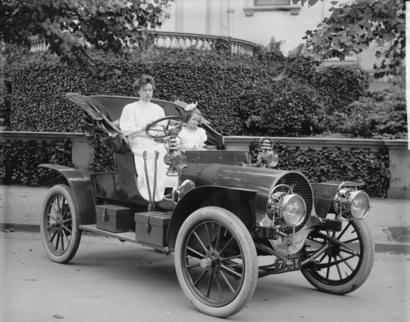
\includegraphics[width=\linewidth]{figures/sample-franklin}
%  \caption{1907 Franklin Model D roadster. Photograph by Harris \&
%    Ewing, Inc. [Public domain], via Wikimedia
%    Commons. (\url{https://goo.gl/VLCRBB}).}
%  \Description{A woman and a girl in white dresses sit in an open car.}
%\end{figure}
%
%Your figures should contain a caption which describes the figure to
%the reader.
%
%Figure captions are placed {\itshape below} the figure.
%
%Every figure should also have a figure description unless it is purely
%decorative. These descriptions convey what’s in the image to someone
%who cannot see it. They are also used by search engine crawlers for
%indexing images, and when images cannot be loaded.
%
%A figure description must be unformatted plain text less than 2000
%characters long (including spaces).  {\bfseries Figure descriptions
%  should not repeat the figure caption – their purpose is to capture
%  important information that is not already provided in the caption or
%  the main text of the paper.} For figures that convey important and
%complex new information, a short text description may not be
%adequate. More complex alternative descriptions can be placed in an
%appendix and referenced in a short figure description. For example,
%provide a data table capturing the information in a bar chart, or a
%structured list representing a graph.  For additional information
%regarding how best to write figure descriptions and why doing this is
%so important, please see
%\url{https://www.acm.org/publications/taps/describing-figures/}.
%
%\subsection{The ``Teaser Figure''}
%
%A ``teaser figure'' is an image, or set of images in one figure, that
%are placed after all author and affiliation information, and before
%the body of the article, spanning the page. If you wish to have such a
%figure in your article, place the command immediately before the
%\verb|\maketitle| command:
%\begin{verbatim}
%  \begin{teaserfigure}
%    \includegraphics[width=\textwidth]{sampleteaser}
%    \caption{figure caption}
%    \Description{figure description}
%  \end{teaserfigure}
%\end{verbatim}
%
%\section{Citations and Bibliographies}
%
%The use of \BibTeX\ for the preparation and formatting of one's
%references is strongly recommended. Authors' names should be complete
%--- use full first names (``Donald E. Knuth'') not initials
%(``D. E. Knuth'') --- and the salient identifying features of a
%reference should be included: title, year, volume, number, pages,
%article DOI, etc.
%
%The bibliography is included in your source document with these two
%commands, placed just before the \verb|\end{document}| command:
%\begin{verbatim}
%  \bibliographystyle{ACM-Reference-Format}
%  \bibliography{bibfile}
%\end{verbatim}
%where ``\verb|bibfile|'' is the name, without the ``\verb|.bib|''
%suffix, of the \BibTeX\ file.
%
%Citations and references are numbered by default. A small number of
%ACM publications have citations and references formatted in the
%``author year'' style; for these exceptions, please include this
%command in the {\bfseries preamble} (before the command
%``\verb|\begin{document}|'') of your \LaTeX\ source:
%\begin{verbatim}
%  \citestyle{acmauthoryear}
%\end{verbatim}
%
%  Some examples.  A paginated journal article \cite{Abril07}, an
%  enumerated journal article \cite{Cohen07}, a reference to an entire
%  issue \cite{JCohen96}, a monograph (whole book) \cite{Kosiur01}, a
%  monograph/whole book in a series (see 2a in spec. document)
%  \cite{Harel79}, a divisible-book such as an anthology or compilation
%  \cite{Editor00} followed by the same example, however we only output
%  the series if the volume number is given \cite{Editor00a} (so
%  Editor00a's series should NOT be present since it has no vol. no.),
%  a chapter in a divisible book \cite{Spector90}, a chapter in a
%  divisible book in a series \cite{Douglass98}, a multi-volume work as
%  book \cite{Knuth97}, a couple of articles in a proceedings (of a
%  conference, symposium, workshop for example) (paginated proceedings
%  article) \cite{Andler79, Hagerup1993}, a proceedings article with
%  all possible elements \cite{Smith10}, an example of an enumerated
%  proceedings article \cite{VanGundy07}, an informally published work
%  \cite{Harel78}, a couple of preprints \cite{Bornmann2019,
%    AnzarootPBM14}, a doctoral dissertation \cite{Clarkson85}, a
%  master's thesis: \cite{anisi03}, an online document / world wide web
%  resource \cite{Thornburg01, Ablamowicz07, Poker06}, a video game
%  (Case 1) \cite{Obama08} and (Case 2) \cite{Novak03} and \cite{Lee05}
%  and (Case 3) a patent \cite{JoeScientist001}, work accepted for
%  publication \cite{rous08}, 'YYYYb'-test for prolific author
%  \cite{SaeediMEJ10} and \cite{SaeediJETC10}. Other cites might
%  contain 'duplicate' DOI and URLs (some SIAM articles)
%  \cite{Kirschmer:2010:AEI:1958016.1958018}. Boris / Barbara Beeton:
%  multi-volume works as books \cite{MR781536} and \cite{MR781537}. A
%  couple of citations with DOIs:
%  \cite{2004:ITE:1009386.1010128,Kirschmer:2010:AEI:1958016.1958018}. Online
%  citations: \cite{TUGInstmem, Thornburg01, CTANacmart}. Artifacts:
%  \cite{R} and \cite{UMassCitations}.
%

%%
%% The next two lines define the bibliography style to be used, and
%% the bibliography file.
%\bibliographystyle{ACM-Reference-Format}
%\bibliography{bibliography}

\end{document}
\endinput
%%
%% End of file `sample-sigconf.tex'.
